% rubber: set program xelatex

% The theme used for this presentation is matze's mtheme, which can be
% found at https://github.com/matze/mtheme

\newif\ifhandout
\newif\ifextended

\handoutfalse
%\handouttrue

\extendedfalse
%\extendedtrue

\ifhandout
    \documentclass[12 pt, compress, handout, intlimits]{beamer}

    \setbeamertemplate{note page}[plain]

    \setbeameroption{show notes}% on second screen=bottom}
\else

    \documentclass[12 pt, compress, intlimits]{beamer}

\fi

\usetheme{metropolis}

\usepackage{mymacros}
\usepackage[retainorgcmds]{IEEEtrantools}
\setlength{\IEEEnormaljot}{9pt}

\renewcommand{\d}{\operatorname{d}\!}
\renewcommand{\L}{\mathcal{L}}
\renewcommand{\B}{\mathcal{B}}
\newcommand{\inprod}[2]{\left\langle {#1}, {#2} \right\rangle}
\newcommand{\conj}[1]{\overline{#1}}

\usepackage{graphicx}
\usepackage{booktabs}
\usepackage[scale=2]{ccicons}
\usepackage{array}
\usepackage{tabularx}

\usepackage{xcolor}
\usepackage{mathtools}
\usepackage{empheq}

\renewcommand{\tabularxcolumn}[1]{>{\normalsize}m{#1}}

\newcommand{\highlight}[1]{\colorbox{mLightBrown!65}{$\displaystyle{#1}$}}
\newcommand{\mygreenbox}[1]{\colorbox{mLightBrown!65}{\hspace{1em}#1\hspace{1em}}}
\newcommand*\widefbox[1]{\fbox{\hspace{1em}#1\hspace{1em}}}


%\usepgfplotslibrary{dateplot}

%\usefonttheme[onlymath]{serif}
%\usepackage{eulervm}
%\usepackage{arevmath}
%\renewcommand{\vect}[1]{\vec{#1}}
\renewcommand{\L}{\mathcal{L}}
\newcommand{\ft}[1]{\tilde{#1}}
\newcommand{\rinprod}[2]{\left\langle {#1}, {#2} \right\rangle_r}
\newcommand{\pinprod}[2]{\left\langle {#1}, {#2} \right\rangle_p}

\useinnertheme{circles}

\setbeamercovered{transparent}

\title{Green's functions}
\subtitle{A short introduction}
\date{\today}
\author{Chris Deimert}
\institute{Department of Electrical and Computer Engineering, University of Calgary}

\begin{document}

\maketitle

\note{
    \begin{itemize}
    \item
        This is intended as a short introduction to Green's functions for electrical engineers.
    \item
        Basic idea of Green's functions is simple, but there is a huge amount of theory for actually calculating and using them.
    \item
        We won't be able to cover much here, but we'll try to focus on building a solid foundation and understanding of Green's functions.
    \item
        Suggested further reading is provided at the end.
    \end{itemize}
}

\begin{frame}[fragile]
    \frametitle{Outline}
    \tableofcontents
\end{frame}

\note{
\begin{enumerate}
\item
    Basic idea of Green's functions.
\item
    Simplest method for solving the Green's function equation.
\item
    How to use the Green's function to solve a problem with boundary conditions. (Biggest section!)
\item
    Useful properties of Green's functions for special types of problems.
\item
    Summary and suggested further reading.
\end{enumerate}

}

\section{Basic idea}
\label{sec:basic_idea}

\note{
\begin{itemize}
\item
    The basic idea of Green's functions is really simple.
    You've actually used them before!
\end{itemize}
}

\begin{frame}[fragile]
    \frametitle{What is a Green's function?}
    
    Linear equation to solve:
    \begin{align*}
        \L u(x) &= f(x)
    \end{align*}
    
    \pause

    Green's function is the \textbf{impulse response}:
    \begin{align*}
        \L G(x,x') &= \delta(x - x')
    \end{align*}

\end{frame}

\note{
\begin{itemize}
\item
    Most electromagnetics problems are described by linear (differential) equations with some source/driving function $ f(x) $.
\item
    The Green's function is the solution when the source $ f(x) $ is set equal to an impulse (delta function) located at $ x' $.
\item
    Can think of it as a generalization of the familiar impulse response from signal processing.
\end{itemize}
}

\begin{frame}[fragile]
    \frametitle{Why is it useful?}
    
    \begin{align*}
        \delta(x - x') &\xrightarrow{\quad \L^{-1} \quad} G(x,x')
    \end{align*}
 
    \pause

    \begin{align*}
        f(x) = \int \delta(x - x') f(x') \d x \xrightarrow{\quad \L^{-1} \quad} \int G(x,x') f(x') \d x
    \end{align*}
    
\end{frame}

\note{
\begin{itemize}
\item
    Once we know the Green's function for a problem, we can find the solution for any source $ f(x) $.
\item
    Impulses $ \delta(x - x') $ produce a response $ G(x,x') $.
\item
    We can split the source $ f(x) $ up into a sum (integral) of impulses $ \delta(x - x') $.
\item
    Then the response to $ f(x) $ is just a weighted sum (integral) of impulse responses.
\end{itemize}
}

\begin{frame}[fragile]
    \frametitle{Why is it useful?}

    \begin{align*}
        \L u(x) &= f(x)
    \end{align*}
    \begin{align*}
        \L G(x,x') &= \delta(x - x')
    \end{align*}
    \begin{empheq}[box=\widefbox]{align*}
        u(x) = \int G(x,x') f(x') \d x
    \end{empheq}
    \begin{flushright}\scriptsize{(Some conditions apply.)}\end{flushright}

\end{frame}

\note{
\begin{itemize}
\item
    Once we know the Green's function, we have an explicit formula for the solution $ u(x) $ for any source function $ f(x) $.
\item
    Beware the fine print! 
    This formula actually only works under certain assumptions about the boundary conditions.
\item
    We'll deal with the more general approach later.
    For now, we'll use this simple version to get the key idea across.
\end{itemize}
}

\begin{frame}[fragile]
    \frametitle{Familiar Green's functions}

    Impulse response of a linear time-invariant system:
    \begin{align*}
        y(t) &= \int_{-\infty}^{\infty} x(t') \alert{h(t - t')} \d t'
    \end{align*}

\end{frame}

\note{
\begin{itemize}
\item
    In electrical engineering, we've seen Green's functions before.
\item
    Impulse response $ h(t - t') $ from linear system theory is an example of a Green's function.
    \begin{align*}
        G(t,t')  = h(t - t')
    \end{align*}
\item
    Output $ y(t) $ is given by convolution of the impulse $ h(t) $ with the input $ x(t) $.
\end{itemize}
}

\begin{frame}[fragile]
    \frametitle{Familiar Green's functions}

    Poisson's equation:
    \begin{align*}
        \nabla^2 V(\vect{r}) &= - \frac{\rho(\vect{r})}{\epsilon_0}
    \end{align*}
    \begin{align*}
        V(\vect{r}) &= \iiint \alert{\frac{1}{4 \pi \epsilon_0 \left| \vect{r} - \vect{r}' \right|}} \rho(\vect{r}') \d^3 \vect{r}'
    \end{align*}
\end{frame}

\note{
    \begin{itemize}
    \item
        Green's function for Poisson's equation is
        \begin{align*}
            G(\vect{r}, \vect{r}') &= \frac{1}{4 \pi \epsilon_0 \left| \vect{r} - \vect{r}' \right|}
        \end{align*}
    \item
        The Green's function is the potential created by a point (impulse) charge.
    \end{itemize}
}

\begin{frame}[fragile]
    \frametitle{Familiar Green's functions}
    
    Helmholtz equation:
    \begin{align*}
        \left( \nabla^2 + k^2 \right) A_z(\vect{r}) &= -J_z(\vect{r})
    \end{align*}
    \begin{align*}
        A_z(\vect{r}) &= \iiint \alert{\frac{e^{-jk \left| \vect{r} - \vect{r}' \right|}}{4 \pi \left| \vect{r} - \vect{r}' \right|}} J_z\left( \vect{r}' \right) \d^3 \vect{r}'
    \end{align*}
\end{frame}

\note{
    \begin{itemize}
    \item
        Green's function for the Helmholtz equation is
        \begin{align*}
            G(\vect{r}, \vect{r}') &= \frac{e^{-jk \left| \vect{r} - \vect{r}' \right|}}{4 \pi \left| \vect{r} - \vect{r}' \right|}
        \end{align*}
    \item
        The Green's function is the potential created by a point (impulse) current.
    \end{itemize}
}

\begin{frame}[fragile]
    \frametitle{Familiar Green's functions}
    
    Green's functions let us:
    \begin{itemize}
    \item
        Derive and understand these expressions.
    \item
        Generalize to other problems and boundary conditions.
    \end{itemize}
    
\end{frame}

\note{
\begin{itemize}
\item
    With Green's function theory, we learn how to derive the above expressions and understand them a little more rigorously. (Though we won't have time to derive the 3D ones here.)
\item
    In addition, Green's function theory allows us to deal with different boundary conditions.
    The solutions to the Poisson and Helmholtz equations above assume free space (boundaries at infinity).
    Green's functions would allow us to, e.g., find the response to a current source inside a specific waveguide.
\end{itemize}
}

\section{Finding the Green's function}
\label{sec:finding_the_green_s_function}
\note{
\begin{itemize}
\item
    In this section, we'll look at one of the simplest methods for actually solving the Green's function problem.
\item
    Often called the \emph{direct method}.
\end{itemize}
}

\begin{frame}[fragile]
    \frametitle{A simple example}

    Original problem:
    \begin{align*}
        \frac{\d^2 u(x)}{\d x^2} - k^2 u(x) &= f(x)
    \end{align*}
    
    Green's function problem:
    \begin{align*}
        \frac{\d^2 G(x, x')}{\d x^2} - k^2 G(x,x') &= \delta(x - x')
    \end{align*}
    

\end{frame}

\note{
\begin{itemize}
\item
    Let's start off by looking at a simple example.
\item
    This problem is similar to a simple harmonic oscillator, but the negative sign means we expect lossy behaviour rather than oscillation.
\item
    We won't worry much about boundary conditions yet, we'll just look for solutions that don't blow up at $ x = \pm \infty $.
\item
    If we can find the Green's function, then we can find the solution to the original problem for any $ f(x) $.
\item
    But the Green's function problem looks hard! 
    The point of this example is to demonstrate that we can actually solve it.
\end{itemize}
}

\begin{frame}[fragile]
    \frametitle{A simple example}

    For $ x \neq x' $
    \begin{align*}
        \frac{\d^2 G(x, x')}{\d x^2} - k^2 G(x,x') &= 0
    \end{align*}
    
    \pause
    So we have
    \begin{align*}
        G(x,x') &= 
        \begin{cases} 
            A e^{+k (x - x')} & \text{for } x < x'
            \\
            B e^{-k (x - x')} & \text{for } x > x'
        \end{cases}
    \end{align*}
    
    
\end{frame}

\note{
    \begin{itemize}
    \item
        Key thing to notice is that the source is concentrated at $ x = x' $.
    \item
        So for $ x > x' $ and $ x < x' $, we expect the solutions to look like those of the source-free equation.
    \item
        To keep the solutions finite, we expect exponential growth before $ x = x' $ and exponential decay afterward.
    \item
        Now, how do we find the constants $ A $ and $ B $?
    \end{itemize}
}

\begin{frame}[fragile]
    \frametitle{A simple example}

    \begin{align*}
        \frac{\d^2 G(x,x')}{\d x^2} - k^2 G(x,x') &= \delta(x - x')
    \end{align*}

    \pause
    Continuity of the Green's function:
    \begin{align*}
        \lim_{\epsilon \to 0} \left[ G(x'+\epsilon, x') - G(x' - \epsilon, x') \right] = 0
    \end{align*}

\end{frame}

\note{
\begin{itemize}
\item
    How continuous do we expect our Green's function to be?
\item
    If $ G(x,x') $ is discontinuous (like a step function), then $ \d G / \d x $ will behave like a delta function and $ \d^2 G / \d x^2 $ will behave like a delta function derivative. No good!
\item
    So we expect $ G(x,x') $ to be continuous.
\item
    That gives us one condition we can use to find $ A $ and $ B $. (In fact, it tells us that $ A = B $.)
\end{itemize}
}

\begin{frame}[fragile]
    \frametitle{A simple example}
 
    \begin{align*}
        \alt<2->{\int_{x'-\epsilon}^{x'+\epsilon} \left[ \frac{\d^2 G(x, x')}{\d x^2} - k^2 G(x,x') \right] \d x &= \int_{x'-\epsilon}^{x'+\epsilon} \delta(x - x') \d x}{\frac{\d^2 G(x, x')}{\d x^2} - k^2 G(x,x') = \delta(x - x')}
    \end{align*}

    \pause
    \pause
    Discontinuity condition:
    \begin{align*}
        \lim_{\epsilon \to 0} \left[ \left. \frac{\d G}{\d x}\right|_{x = x' + \epsilon} - \left. \frac{\d G}{\d x} \right|_{x = x' - \epsilon} \right] &= 1
    \end{align*}
    

\end{frame}

\note{
    \begin{itemize}
    \item
        But what if the derivative $ \d G / \d x $ is discontinuous?
    \item
        Then $ \d^2 G / \d x^2 $ is like a delta function.
        But that's fine, because we have a delta function on the right hand side too.
    \item
        We can find exactly how discontinuous the derivative is by integrating over a small interval around $ x' $.
    \item
        In the limit of $ \epsilon \to 0 $, the second integral vanishes because $ G(x,x') $ is continuous.
    \item
        The first integral is an integral of a derivative, so we can use the fundamental theorem of calculus.
        The result is a \emph{discontinuity condition for the derivative.}
    \end{itemize}
}

\begin{frame}[fragile]
    \frametitle{A simple example}

    \begin{align*}
        G(x,x') &= 
        \begin{cases} 
            A e^{+k (x - x')} & \text{for } x < x'
            \\
            B e^{-k (x - x')} & \text{for } x > x'
        \end{cases}
    \end{align*}
    
    Continuity of $ G(x,x') $:
    \begin{align*}
        A &= B
    \end{align*}

    Discontinuity of $ \dfrac{\d G(x,x')}{\d x} $:
    \begin{align*}
        k A + k B = 1
    \end{align*}
    
\end{frame}

\note{
\begin{itemize}
\item
    Applying our two conditions, we can solve for $ A $ and $ B $.
    We find
    \begin{align*}
        A = B = \frac{1}{2 k}
    \end{align*}
    
\end{itemize}
}

\begin{frame}[fragile]
    \frametitle{A simple example}
    Solving, our Green's function is
    \begin{align*}
        G(x,x') &= \frac{1}{2k} 
        \begin{dcases} 
            e^{+k (x - x')} & \text{for } x < x'
            \\
            e^{-k (x - x')} & \text{for } x > x'
        \end{dcases}
    \end{align*}
    Or, more compactly:
    \begin{empheq}[box=\widefbox]{align*}
        G(x, x') = \frac{e^{k |x - x'|}}{2 k}
    \end{empheq}
    

\end{frame}

\note{
}

\begin{frame}[fragile]
    \frametitle{A simple example}

    Original problem:
    \begin{align*}
        \frac{\d^2 u(x)}{\d x^2} - k^2 u(x) &= f(x)
    \end{align*}

    Solution:
    \begin{align*}
        u(x) &= \int_{-\infty}^{\infty} f(x') \frac{e^{k|x - x'|}}{2k} \d x'
    \end{align*}
    
\end{frame}

\note{
\begin{itemize}
\item
    Now that we have the Green's function, we can construct the solution to our original problem for any forcing function $ f(x) $.
\item
    Caution: remember the fine print from before. 
    This solution only works with certain assumptions about boundary conditions.
    (More on this to come!)
\end{itemize}
}

\begin{frame}[fragile]
    \frametitle{General approach}

    Direct solution:
    \begin{itemize}
    \item
        $ G(x,x') $ obeys source-free equation for $ x \neq x' $.
    \item
        $ G(x,x') $ and its derivatives are continuous or discontinuous at $ x = x' $.
    \end{itemize}
    
\end{frame}

\note{
    \begin{itemize}
    \item
        Write down the source-free solution for $ x \neq x' $: usually has a few unknown coefficients.
    \item
        Examine the equation to find continuity/discontinuity requirements for $ G(x,x') $ and its derivatives.
        (Most books on Green's functions provide these requirements for general Sturm-Liouville problems.)
    \item
        This approach is great if it works.
        Unfortunately, it doesn't always work (especially in 3D problems).
    \item
        We'll briefly look at an alternative solution method later using eigenvalues and eigenfunctions, but this still just scratches the surface. 
        See the references provided at the end.
    \end{itemize}
}

\section{Constructing the solution}
\label{sec:constructing_the_solution}

\note{}

\begin{frame}[fragile]
    \frametitle{Constructing the solution}

    \begin{align*}
        u(x) &= \int G(x,x') f(x') \d x'
    \end{align*}
    
    \begin{center}Can we prove/generalize this?\end{center}
    
\end{frame}

\note{
\begin{itemize}
\item
    In the introduction, we showed non-rigorously how to construct a solution from the Green's function.
    To keep things simpler, we ignored boundary conditions.
\item
    Here, we'll look at how to properly construct a solution from the Green's function when boundary conditions are involved.
\item
    Our approach is quite challenging compared to a lot of books on the subject. 
    The advantage is that we'll deal with some subtleties that can otherwise lead to confusion.
\item
    For approaches similar to the one in this section, see Dudley, Morse and Feshbach, or Gerlach.
\end{itemize}
}

\begin{frame}[fragile]
    \frametitle{Adjoint operators}

    Inner product:
    \begin{align*}
        \inprod{u}{v} &= \int_a^b u(x) \conj{v}(x) \d x
    \end{align*}
    
    Adjoint operator $ \L^* $:
    \begin{align*}
        \inprod{\L u}{v} &= \inprod{u}{\L^* v}
    \end{align*}
   

\end{frame}

\note{
\begin{itemize}
\item
    Underpinning our approach is the idea of an adjoint operator.
\item
    Start with an inner product (for 1D problems, usually the one shown).
    Note that $ \conj{v} $ is the complex conjugate of $ v $.
\item
    If $ \L $ is a linear operator, then its adjoint $ \L^* $ is defined as the operator which satisfies
    \begin{align*}
        \inprod{\L u}{v} &= \inprod{u}{\L^* v}
        \\
        \Longrightarrow \quad \int_a^b (\L u) v^* \d x &= \int_a^b u \conj{(\L^* v)} \d x
    \end{align*}
\item
    Roughly, $ \L^* $ is what appears if we try to move $ \L $ into the other slot of the inner product. 
\end{itemize}
}

\begin{frame}[fragile]
    \frametitle{Adjoint boundary conditions}
    
    \begin{align*}
        \inprod{\L u}{v} &= \inprod{u}{\L^* v} \longrightarrow \text{Only for certain $ u, v $ !}
    \end{align*}

    Adjoint boundary conditions:
    \begin{align*}
        \B_i[u] &= 0; \qquad \B_i^*[v] = 0
    \end{align*}
    
    Otherwise
    \begin{align*}
        \inprod{\L u}{v} &= \inprod{u}{\L^* v} + \underbrace{J(u,\conj{v})}_{\text{Conjunct}} \Big|_a^b
    \end{align*}
    

\end{frame}

\note{
\begin{itemize}
\item
    The adjoint is only truly the adjoint (i.e., $ \inprod{\L u}{v} = \inprod{u}{\L^* v} $) for certain functions $ u $ and $ v $.
    (Mathematically, when $ \L $ and $ \L^* $ are unbounded operators, they do not necessarily share the same \emph{domain}, and we need to consider that.)
\item
    This is where boundary conditions come in. 
    Specifically, if $ u $ obeys some boundary conditions $ \B_i[u] = 0 $, then $ v $ has to obey some adjoint boundary conditions $ \B_i^*[v] = 0 $.
\item
    Note on notation: $ \B_i[u] = 0 $ means that some linear combination of $ u $ and its derivatives are set equal to zero at the boundaries.
\item
    If $ \B_i[u] = 0 $ and $ \B_i^*[v] = 0 $ are not satisfied, then the adjoint equation almost holds, but we get an extra term $ J(u,v^*) $ called the \emph{conjunct}. It's only evaluated at the boundaries.
\end{itemize}

}

\begin{frame}[fragile]
    \frametitle{Adjoint operators: example}
    \begin{align*}
        \L u(x) &= \left[ \frac{\d^2}{\d x^2} + k^2 \right] u(x)
    \end{align*}

    Want $ \L^* $ so that
    \begin{align*}
        \inprod{\L u}{v} &= \inprod{u}{\L^* v} + J(u, \conj{v})\Big|_a^b
    \end{align*}

\end{frame}

\note{
    \begin{itemize}
    \item
        Let's look at an example: the 1D simple harmonic oscillator.
    \item
        Let's try to find $ \L^* $ without worrying about boundary conditions for now.
        (So we expect the conjunct to appear.)
    \end{itemize}
}

\begin{frame}[fragile]
    \frametitle{Adjoint operators: example}
    
    \begin{align*}
        \inprod{\L u}{v} &= \int_a^b \left[ u'' + k^2 u \right] \conj{v} \d x
        \\
        \inprod{\L u}{v} &= \int_a^b \left[ -u' \conj{v}' + k^2 u \conj{v} \right] \d x + \left[ u' \conj{v} \right]_a^b
        \\
        \inprod{\L u}{v} &= \int_a^b u \left[ \conj{v}^{\prime\prime} + k^2 \conj{v} \right] \d x + \left[ u' \conj{v}  - u \conj{v}' \right]_{a}^{b}
    \end{align*}
    

\end{frame}

\note{
    \begin{itemize}
    \item
        To find the adjoint, let's expand $ \inprod{\L u}{v} $.
    \item
        Use integration by parts twice.
    \end{itemize}
}

\begin{frame}[fragile]
    \frametitle{Adjoint operators: example}

    \begin{align*}
        \inprod{\L u}{v} &= \int_a^b u \left[ \conj{v}^{\prime\prime} + k^2 \conj{v} \right] \d x + \left[ u' \conj{v}  - u \conj{v}' \right]_{a}^{b}
    \end{align*}
    
    Looks like
    \begin{align*}
        \inprod{\L u}{v} &= \inprod{u}{\L^* v} + J(u, \conj{v})\Big|_a^b
    \end{align*}
    with
    \begin{align*}
        \L^* &= \frac{\d^2}{\d x^2} + \conj{k^2}
        \\[4pt]
        J(u,\conj{v}) &= u' \conj{v}  - u \conj{v}'
    \end{align*}
    
\end{frame}

\note{
\begin{itemize}
\item
    After integration by parts, we can read off the adjoint operator and the conjunct.
\item
    So in this case, the adjoint operator is the almost the same as the original operator, but there's an extra complex conjugate.
    If $ k $ is real, then $ \L = \L^* $.
\end{itemize}
}

\begin{frame}[fragile]
    \frametitle{Adjoint operators: example}

    For
    \begin{align*}
        \inprod{\L u}{v} &= \inprod{u}{\L^* v}
    \end{align*}
    must have
    \begin{align*}
        J(u,\conj{v})\Big|_a^b &= 0
        \\
        \left[u' \conj{v}  - u \conj{v}'\right]_a^b &= 0
    \end{align*}
    \begin{align*}
        u'(b) \conj{v}(b) - u(b) \conj{v}'(b) - u'(a) \conj{v}(a) + u(a) \conj{v}'(a) = 0
    \end{align*}
    
\end{frame}

\note{
\begin{itemize}
\item
    Now let's look at adjoint boundary conditions.
\item
    For $ \L^* $ to be a true adjoint, we need the conjunct to be zero.
\item
    Let's expand the conjunct for this particular example.
\end{itemize}
}

\begin{frame}[fragile]
    \frametitle{Adjoint operators: example}

    \begin{align*}
        u'(b) \conj{v}(b) - u(b) \conj{v}'(b) - u'(a) \conj{v}(a) + u(a) \conj{v}'(a) = 0
    \end{align*}

    Boundary conditions:
    \begin{align*}
        \begin{array}{c}
        \B_1[u] = u(a) = 0
        \\
        \B_2[u] = u(b) = 0
        \end{array}
        \Longrightarrow
        \begin{array}{c}
        \B^*_1[v] = v(a) = 0
        \\
        \B^*_2[v] = v(b) = 0
        \end{array}
    \end{align*}

    \begin{align*}
        \B_i &= \B_i^*
    \end{align*}
    
    
\end{frame}

\note{
\begin{itemize}
\item
    Suppose we have the simple boundary conditions $ u(a) = u(b) = 0 $.
\item
    Then, to make the conjunct zero, we need $ \conj{v}(a) = \conj{v}(b) = 0 $ or $ v(a) = v(b) = 0 $.
\item
    So in this case, the adjoint boundary conditions on $ v $ are the same as the boundary conditions on $ u $.
\item
    Remember what these boundary conditions mean.
    $ \L^* $ is the true adjoint when $ \L $ operates on functions $ u(x) $ which are zero at $ x = a,b $ and $ \L^* $ operates on functions $ v(x) $ which are zero at $ x = a,b $.
\end{itemize}
}

\begin{frame}[fragile]
    \frametitle{Adjoint operators: example}

    \begin{align*}
        u'(b) \conj{v}(b) - u(b) \conj{v}'(b) - u'(a) \conj{v}(a) + u(a) \conj{v}'(a) = 0
    \end{align*}

    Initial conditions:
    \begin{align*}
        \begin{array}{c}
        \B_1[u] = u(a) = 0
        \\
        \B_2[u] = u'(a) = 0
        \end{array}
        \Longrightarrow
        \begin{array}{c}
        \B^*_1[v] = v(b) = 0
        \\
        \B^*_2[v] = v'(b) = 0
        \end{array}
    \end{align*}

    \begin{align*}
        \B_i &\neq \B_i^*
    \end{align*}
    
\end{frame}

\note{
\begin{itemize}
\item
    What if we have initial conditions instead? $ u(a) = u'(a) = 0 $.
\item
    Then, to make the conjunct zero, we need $ v(b) = v'(b) = 0 $.
\item
    So, for initial conditions, the adjoint boundary conditions are \emph{final} conditions.
    $ \B_i \neq \B_i^* $.
\end{itemize}
}


\begin{frame}[fragile]
    \frametitle{Adjoint operators: summary}

    Adjoint operator:
    \begin{align*}
        \inprod{\L u}{v} &= \inprod{u}{\L^* v}
    \end{align*}
    Adjoint boundary conditions:
    \begin{align*}
        \begin{array}{c} \B_i[u] = 0 \\ \B^*_i[v] = 0 \end{array} \Longrightarrow J(u,\conj{v})\Big|_a^b = 0
    \end{align*}
    Otherwise:
    \begin{align*}
        \inprod{\L u}{v} &= \inprod{u}{\L^* v} + J(u,\conj{v}) \Big|_a^b
    \end{align*}
    
    
    
\end{frame}

\note{
\begin{itemize}
\item
    The adjoint operator satisfies $ \inprod{\L u}{v} = \inprod{u}{\L^* v} $.
\item
    This only works for certain $ u,v $, though.
    Specifically, it works when $ u $ obeys boundary conditions and $ v $ obeys adjoint boundary conditions.
\item
    If $ u,v $ do not satisfy these boundary conditions, then $ \L^* $ is not truly the adjoint anymore.
    However, it still nearly obeys the adjoint equation; there's just a leftover conjunct term which depends on the boundary values of $ u, v $ and their derivatives.
\item
    For a lot of things (e.g., using eigenfunction bases) we need this conjunct to be zero.
    But for Green's functions, it will end up being indispensible.
\end{itemize}

}

\begin{frame}[fragile]
    \frametitle{The adjoint Green's function}
 
    Original problem:
    \begin{IEEEeqnarray*}{rClCrCl}
        \L u(x) &=& f(x); &\qquad& \B_i [u(x)] &=& \alpha_i
    \end{IEEEeqnarray*}
    Green's problem:
    \begin{IEEEeqnarray*}{rClCrCl}
        \L G(x,x') &=& \delta(x - x'); &\qquad& \B_i [G(x,x')] &=& 0
    \end{IEEEeqnarray*}
    Adjoint Green's problem:
    \begin{IEEEeqnarray*}{rClCrCl}
        \L^* H(x,x') &=& \delta(x - x'); &\qquad& \B_i^* [H(x,x')] &=& 0
    \end{IEEEeqnarray*}
    
\end{frame}

\note{
\begin{itemize}
\item
    Now we'll be able to deal with boundary conditions properly.
\item
    We define $ G(x,x') $ to obey the same equation as $ u(x) $, but with $ f(x) \to \delta(x - x') $ and $ \alpha_i \to 0 $.
    As before, $ G(x,x') $ is the impulse response.
\item
    In addition, we define a new function $ H(x,x') $ which is called the adjoint Green's function.
    It obeys the adjoint version of the $ G(x,x') $ equation.
\item
    Warning! A lot of textbooks don't distinguish between $ H(x,x') $ and $ G(x,x') $.
    Sometimes the ``Green's function'' in an expression is really the adjoint Green's function.
\end{itemize}
}

\begin{frame}[fragile]
    \frametitle{Constructing solutions: derivation}

    \begin{align*}
        \inprod{\L u(x)}{H(x,x')} &= \inprod{u(x)}{\L^* H(x,x')} + J\big(u(x), \conj{H}(x,x')\big) \Big|_a^b
        \\
        \inprod{f(x)}{H(x,x')} &= \inprod{u(x)}{\delta(x - x')} + J\big(u(x), \conj{H}(x,x')\big) \Big|_a^b
        \\
        \int_a^b f(x) H^*(x,x') \d x &= \int_a^b u(x) \delta(x - x') \d x + J\big(u(x), \conj{H}(x,x')\big) \Big|_a^b
    \end{align*}
    \begin{empheq}[box=\widefbox]{align*}
        u(x') &= \int_a^b f(x) \conj{H}(x,x') \d x - J\big(u(x), \conj{H}(x,x')\big) \Big|_a^b
    \end{empheq}
    
\end{frame}

\note{
    \begin{itemize}
    \item
        To construct the solution $ u(x) $, we take an inner product of $ \L u(x) $ with $ H(x,x') $, and apply our knowledge of adjoints and conjuncts.
    \item
        Then, we use the fact that $ \L u(x) = f(x) $ and $ \L H(x,x') = \delta(x - x') $.
    \item
        After evaluating the inner product terms, we arrive at a fairly general formula which looks somewhat like what we had in the introduction.
        The difference is that it involves the \emph{adjoint} Green's function $ H(x,x') $, and it has an extra conjunct term.
    \item
        We'll deal with the conjunct later.
        For now, let's try to get rid of $ H(x,x') $ and express $ u(x) $ in terms of $ G(x,x') $.
        To do that, we need a relationship between $ H(x,x') $ and $ G(x,x') $.
    \end{itemize}
}

\begin{frame}[fragile]
    \frametitle{Constructing solutions: derivation}

    How are $ G(x,x') $ and $ H(x,x') $ related?
    \begin{align*}
        \inprod{\L G(x,x')}{H(x,x'')} &= \inprod{G(x,x')}{\L^* H(x,x'')}
        \\
        \inprod{\delta(x - x')}{H(x,x'')} &= \inprod{G(x,x')}{\delta(x - x'')}
        \\
        \int_a^b \delta(x - x') \conj{H}(x,x'') \d x &= \int_a^b G(x,x') \delta(x - x'') \d x
        \\
        \conj{H}(x',x'') &= G(x'',x')
    \end{align*}
    \begin{empheq}[box=\widefbox]{align*}
        G(x,x') = \conj{H}(x',x)
    \end{empheq}
    
\end{frame}

\note{
    \begin{itemize}
    \item
        Using the definition of the adjoint problem, we find that there is a simple relationship between $ G(x,x') $ and $ H(x,x') $.
    \item
        Note, in the last example, we had to include the conjunct because $ \B[u] \neq 0 $.
        The boundary conditions and adjoint boundary conditions have to be set to zero to eliminate the conjunct.
        In this case, $ \B[G] = 0 $ and $ \B[H] = 0 $, so the conjunct is eliminated.
    \item
        Also note a surprising result of this: if $ G(x,x') $ obeys the boundary conditions with respect to $ x $, then it automatically obeys the \emph{adjoint} boundary conditions with respect to $ x' $. 
        We'll come back to this idea later.
    \end{itemize}
}

\begin{frame}[fragile]
    \frametitle{Constructing solutions: derivation}

    \begin{align*}
        u(x') &= \int_a^b f(x) \conj{H}(x,x') \d x - J\big(u(x), \conj{H}(x,x')\big) \Big|_a^b
    \end{align*}
    \begin{center}and\end{center}
    \begin{align*}
        G(x,x') = \conj{H}(x',x)
    \end{align*}
    \begin{center}so\end{center}
    \begin{empheq}[box=\widefbox]{align*}
        u(x) &= \int_{a}^{b} f(x') G(x,x') \d x' - J\big( u(x'), G(x,x') \big) \Big|_{x'=a}^b
    \end{empheq}
    
\end{frame}

\note{
\begin{itemize}
\item
    Let's go back to our expression for $ u(x') $ in terms of $ H(x,x') $.
\item
    Using our new relationship $ G(x,x') = \conj{H}(x,x') $, we can rewrite this as an expression for $ u(x) $ in terms of $ G(x,x') $.
    (Note: we switched $ x $ and $ x' $ to make it look a little nicer.)
\item
    So this is the more correct version of what we saw in the introduction.
    If the conjunct happens to be zero, then we get what we had before.
    If not, we have an extra term that depends only on the boundaries.
\item
    In general, the conjunct term deals with the boundary conditions of $ u(x) $.
    It turns out that the boundary conditions act, in some way, like additional sources.
    We'll look more closely at this now through an example.
\end{itemize}
}

\begin{frame}[fragile]
    \frametitle{Example: 1D Poisson equation}

    Original problem:
    \begin{align*}
        \frac{\d^2 V(x)}{\d x^2} &= - \frac{\rho(x)}{\epsilon_0}; \quad \begin{array}{c} V(a) = V_a \\ V(b) = V_b \end{array}
    \end{align*}
    
    Green's problem:
    \begin{align*}
        \frac{\d^2 G(x,x')}{\d x^2} &= \delta(x - x'); \quad \begin{array}{c} G(a,x') = 0 \\ G(b,x') = 0 \end{array}
    \end{align*}

\end{frame}

\note{
\begin{itemize}
\item
    Let's look at a simple 1D voltage problem.
\item
    We have both a charge density $ \rho $ inside the region $ a < x < b $, and we have an applied voltage at the boundaries.
    Intuitively, both of these will affect the voltage in the region.
\item
    In the Green's function problem, we turn the charge density into an impulse function, and we set the applied voltage to zero.
\end{itemize}
}


\begin{frame}[fragile]
    \frametitle{Example: 1D Poisson equation}

    Solution:
    \begin{align*}
        V(x) &= \int_{a}^{b} - \frac{\rho(x')}{\epsilon_0} G(x,x') \d x' - J\big( V(x'), G(x,x') \big) \Big|_{x'=a}^b
    \end{align*}

    Take $ \rho(x) = 0 $ for now.
    \begin{align*}
        V(x) &= - J\big( V(x'), G(x,x') \big) \Big|_{x'=a}^b
    \end{align*}

\end{frame}

\note{
\begin{itemize}
\item
    From our recent results, we can write down the solution for $ V(x) $ in terms of the Green's function.
\item
    Take $ \rho = 0 $ so that we can focus on the boundary conditions for now.
\end{itemize}

}

\begin{frame}[fragile]
    \frametitle{Example: 1D Poisson equation}

    Can show
    \begin{align*}
        \inprod{\L u}{v} &= \int_a^b u'' \conj{v} \d x = \int_a^b u \conj{v}'' \d x + \left[ u' \conj{v} - u \conj{v}' \right]_a^b
    \end{align*}
    
    Comparing with
    \begin{align*}
        \inprod{\L u}{v} &= \inprod{u}{\L^* v} + J(u,v^*) \big|_a^b
    \end{align*}
    we see
    \begin{align*}
        \L^* &= \frac{\d^2}{\d x^2} = \L
        \\[4pt]
        J(u,\conj{v}) &= u' \conj{v} - u \conj{v}'
    \end{align*}
    
\end{frame}

\note{
\begin{itemize}
\item
    To write the solution more explicitly, we need to find the conjunct of the operator $ \L = \d^2 / \d x^2 $.
\item
    As before, use integration by parts and compare with the expected formula.
\end{itemize}

}

\begin{frame}[fragile]
    \frametitle{Example: 1D Poisson equation}

    \begin{IEEEeqnarray*}{rCl}
        V(x) &=& - J\big( V(x'), G(x,x') \big) \Big|_{x'=a}^b
        \\[8pt]
        V(x) &=& \left[ V(x') \frac{\d G(x,x')}{\d x'} - \frac{\d V(x')}{\d x'} G(x,x') \right]_{x'=a}^b
        \\[8pt]
        V(x) &=& V_b \frac{\d G(x,b)}{\d x'} - \frac{\d V(b)}{\d x'} G(x,b) -
        \\[4pt] && - V_a \frac{\d G(x,a)}{\d x'} + \frac{\d V(a)}{\d x'} G(x,a)
    \end{IEEEeqnarray*}
    
\end{frame}

\note{
\begin{itemize}
\item
    Now that we know the conjunct, we can write the solution for $ V(x) $ more explicitly.
\item
    Problem: we don't know $ \d V / \d x $ at the boundaries.
\item
    The adjoint problem saves us, because we can show that $ G(x,b) = G(x,a) = 0 $.
\end{itemize}
}

\begin{frame}[fragile]
    \frametitle{Example: 1D Poisson equation}

    Green's problem:
    \begin{align*}
        \frac{\d^2 G(x,x')}{\d x^2} &= \delta(x - x'); \quad \begin{array}{c} G(a,x') = 0 \\ G(b,x') = 0 \end{array}
    \end{align*}
    
    
    Adjoint Green's problem:
    \begin{align*}
        \frac{\d^2 H(x,x')}{\d x^2} &= \delta(x - x'); \quad \begin{array}{c} H(a,x') = 0 \\ H(b,x') = 0 \end{array}
    \end{align*}

    But $ G(x,x') = \conj{H}(x',x) $ so
    \begin{align*}
        \frac{\d^2 \conj{G}(x,x')}{\d x^{\prime 2}} &= \delta(x - x'); \quad \begin{array}{c} G(x,a) = 0 \\ G(x,b) = 0 \end{array}
    \end{align*}

\end{frame}

\note{
\begin{itemize}
\item
    Back to the adjoint Green's equation.
\item
    Because of the relationship between $ G(x,x') $ and $ H(x,x') $ we see that $ G^*(x,x') $ obeys the adjoint equation with respect to $ x' $.
\item
    More importantly, we see that $ \conj{G}(x,x') $ (and thus $ G(x,x') $) obeys the adjoint boundary conditions with respect to $ x' $.
\item
    So not only do we have $ G(a,x') = G(b,x') = 0 $, we also have $ G(x,a) = G(x,b) = 0 $.
    This is not a trivial or obvious result (at least to me).
\end{itemize}
}

\begin{frame}[fragile]
    \frametitle{Example: 1D Poisson equation}
    
    \begin{IEEEeqnarray*}{rCl}
        V(x) &=& V_b \frac{\d G(x,b)}{\d x'} - \frac{\d V(b)}{\d x'} G(x,b) -
        \\[4pt] && - V_a \frac{\d G(x,a)}{\d x'} + \frac{\d V(a)}{\d x'} G(x,a)
    \end{IEEEeqnarray*}
    With $ G(x,a) = G(x,b) = 0 $, we have
    \begin{empheq}[box=\widefbox]{align*}
        V(x) &= V_b \frac{\d G(x,b)}{\d x'} - V_a \frac{\d G(x,a)}{\d x'} 
    \end{empheq}
    

\end{frame}

\note{
\begin{itemize}
\item
    Using the fact that $ G(x,x') $ obeys the adjoint boundary conditions with respect to $ x' $, we can eliminate the unknown values and simplify our result.
\item
    Now we have an explicit solution for $ V(x) $ given any boundary conditions $ V(a) = V_a $ and $ V(b) = V_b $.
\item
    Further, we see that the solution only depends on the Green's function.
    It's as if the non-zero boundary conditions $ V_a, V_b $ act like additional sources whose response is given by the Green's function.
\end{itemize}

}

\begin{frame}[fragile]
    \frametitle{Example: 1D Poisson equation}
    
    Full solution with $ \rho(x) $:
    \begin{align*}
        \Aboxed{V(x) = \int_a^b - \frac{\rho(x')}{\epsilon_0} G(x,x') \d x' + V_b \frac{\d G(x,b)}{\d x'} - V_a \frac{\d G(x,a)}{\d x'}}
    \end{align*}

\end{frame}

\note{
\begin{itemize}
\item
    Putting back our charge distribution $ \rho(x) $, we get a full solution for any charge distribution and boundary conditions.
\item
    The first part gives the voltage produced by the charge distribution $ \rho(x) $.
    The last two parts give the voltage produced by the boundary conditions $ V_a, V_b $.
\item
    The response to \emph{both} of these sources of voltage is given by the Green's function!
\item
    For those familiar with the derivative of the delta function, this can be written in an even more suggestive form:
    \begin{align*}
        V(x) &= \int_a^b \left[ - \frac{\rho(x)}{\epsilon_0} - V_b \delta'(x' - b) + V_a \delta'(x' - a) \right] G(x,x') \d x'
    \end{align*}
    
\end{itemize}

}

\begin{frame}[fragile]
    \frametitle{Solving problems with Green's functions}
    \begin{align*}
        \text{Given:} \quad \L u(x) = f(x); \quad \B_i[u(x)] = \alpha_i
    \end{align*}
    \vspace{-12pt}
    \begin{enumerate}
    \item
        Solve Green's problem
        \begin{align*}
            \L G(x,x') = \delta(x - x'); \quad \B_i[G(x,x')] = 0
        \end{align*}
    \item
        Find $ \L^* $, $ \B_i^* $, and $ J(u,\conj{v}) $ from $ \inprod{\L u}{v} $.
    \item
        Solution is
        \begin{align*}
            u(x) &= \int_{a}^{b} f(x') G(x,x') \d x' - J\big( u(x'), G(x,x') \big) \Big|_{x'=a}^b
        \end{align*}
    \item
        Simplify using $ \B^*[G(x,x')] = 0 $ (with respect to $ x' $).
    \end{enumerate}
    
\end{frame}

\note{
Now let's look at the general process for solving a boundary value problem with a source.
\begin{enumerate}
\item
    Set up the Green's function equation by setting the source to $ \delta(x - x') $ and the boundary conditions to zero.
    Solve this to find the Green's function.
\item
    Find $ \L^* $, $ \B_i^* $, and $ J(u,\conj{v}) $ by expanding the inner product $ \inprod{\L u}{v} $ (usually using integration by parts).
\item
    Write down the solution.
\item
    Unknown boundary values of $ u(x) $ will appear in the conjunct term.
    Eliminate them using the fact that $ G(x,x') $ obeys the adjoint boundary conditions with respect to $ x' $.
\end{enumerate}
}

\begin{frame}[fragile]
    \frametitle{Solving 3D problems with Green's functions}
 
    \begin{align*}
        \text{Given:} \quad \L u(\vect{r}) = f(\vect{r}); \quad \B_i[u(\vect{r})] = \alpha_i
    \end{align*}
    \vspace{-12pt}
    \begin{enumerate}
    \item
        Solve Green's problem
        \begin{align*}
            \L G(\vect{r},\vect{r}') = \delta(\vect{r} - \vect{r}'); \quad \B_i[G(\vect{r},\vect{r}')] = 0
        \end{align*}
    \item
        Find $ \L^* $, $ \B^* $, and $ J(u,\conj{v}) $ from $ \inprod{\L u}{v} $.
    \item
        Solution is
        \begin{align*}
            u(\vect{r}) &= \int_{V} f(\vect{r}') G(\vect{r},\vect{r}') \d^3 \vect{r}' - \oint_{\partial V} \vect{J}\big( u(\vect{r}'), G(\vect{r},\vect{r}') \big) \cdot \d \vect{s}
        \end{align*}
    \item
        Simplify using $ \B^*[G(\vect{r},\vect{r}')] = 0 $ (with respect to $ \vect{r}' $).
    \end{enumerate}
       
\end{frame}

\note{
\begin{itemize}
\item
    Great thing about our approach is that it's easily extended to 3D. 
\item
    Inner product is now a volume integral over the region of interest ($ V $).
    Have to use 3D versions of integration by parts (e.g., Green's identities) to find $ \L^* $, $ J(u,\conj{v}) $ and $ \B_i^* $.
\item
    The conjunct is now vector-valued, and it must be integrated over the surface of $ V $ (denoted $ \partial V $).
\item
    Still have the same interpretation though.
    The first (volume) integral is the contribution from the source $ f(\vect{r}) $.
    The second (surface) integral is the contribution from the non-zero boundary conditions.
\end{itemize}
}

\begin{frame}[fragile]
    \frametitle{Constructing the solution}
    Comments:
    \begin{itemize}
    \item
        Calculating Green's functions is not trivial.
    \item
        Adjoint approach is difficult, but offers clarity.
    \end{itemize}
    
\end{frame}

\note{
\begin{itemize}
\item
    Step 1 of our approach (calculate the Green's function) can be difficult: especially in 3D.
    Learning these techniques is time-consuming, but we now have a solid foundation with which to understand them.
\item
    Our approach was not the easiest, but note the critical role played by the adjoint, both in the derivation and the final solution method.
\item
    Though some authors don't talk about adjoints, they still use these ideas.
    E.g., often the ``Green's function'' used in 3D problems is actually the \emph{adjoint} Green's function. (Can be confusing!)
\end{itemize}
}

\section{Special properties}
\label{sec:special_properties}

\note{
\begin{itemize}
\item
    The behaviour of the Green's function is shaped by the type of problem we're trying to solve.
\item
    In this section, we'll see how a lot of properties of problems are tied to properties of the Green's function.
\end{itemize}
}

\begin{frame}[fragile]
    \frametitle{Self-adjointness}

    If $ \L = \L^* $ and $ \B_i = \B_i^* $, then
    \begin{align*}
        G(x,x') &= \conj{G}(x',x)
    \end{align*}
    
\end{frame}

\note{
\begin{itemize}
\item
    Self-adjointness is equivalent to conjugate symmetry of the Green's function.
\item
    If a problem is self-adjoint, then the adjoint Green's function $ H(x,x') $ is the same as the Green's function $ G(x,x') $.
    Then, using a result from before, we find that $ G(x,x') = \conj{G}(x,x') $.
\end{itemize}
}

\begin{frame}[fragile]
    \frametitle{Reciprocity}
    
    Reciprocity in the frequency-domain:
    \begin{align*}
        G(\vect{r}, \vect{r}') &= G(\vect{r}', \vect{r})
    \end{align*}

\end{frame}

\note{
\begin{itemize}
\item
    The notion of reciprocity in electromagnetism can be tied to this property of the Green's function.
\item
    In the frequency-domain, the Green's function is symmetric under interchange of $ \vect{r}, \vect{r}' $ (no complex conjugate!).
    It can be shown that this is equivalent to reciprocity.
    (See Collin for a more thorough discussion using dyadic Green's functions.)
\item
    Mathematically, frequency-domain reciprocity is related to the pseudo-inner product
    \begin{align*}
        \pinprod{u}{v} &= \iiint u(\vect{r}) v(\vect{r}) \d^3 \vect{r}
    \end{align*}
    and operators which are ``self-adjoint'' under it:
    \begin{align*}
        \pinprod{\L u}{v} &= \pinprod{u}{\L v}
    \end{align*}
    
\end{itemize}
}

\begin{frame}[fragile]
    \frametitle{Reciprocity}

    \vspace{14pt}
    Reciprocity in the time-domain:
    \begin{align*}
        G(\vect{r}, t; \vect{r}', -t') &= G(\vect{r}', t'; \vect{r}, -t)
    \end{align*}
    \vspace{-26pt}
    \begin{figure}
        \centering
    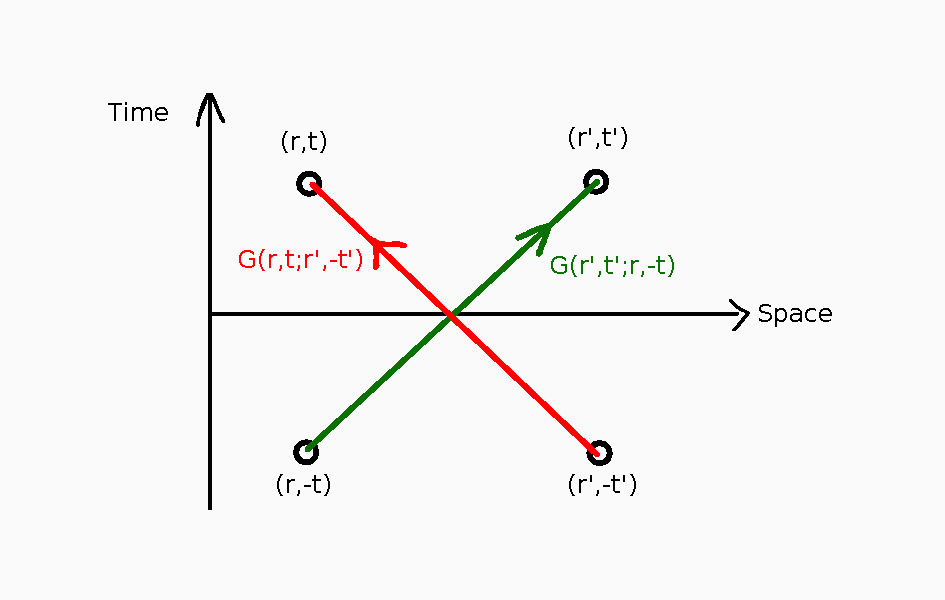
\includegraphics[width=0.9\textwidth]{Reciprocity.pdf}
    \end{figure}
    
\end{frame}

\note{
\begin{itemize}
\item
    In the time-domain, the Green's function is symmetric, but with an added minus sign on the time variables.
    This is because of causality (see Morse and Feshbach).
\item
    Think of $ G(\vect{r}, t; \vect{r}', t') $ as having an impulse at $ (\vect{r}', t') $ and measuring it at $ (\vect{r}, t) $.
    Then reciprocity shows that interchanging sources and measurements leads to identical results.
\item
    Mathematically, time-domain reciprocity related to the pseudo-inner product
    \begin{align*}
        \pinprod{u}{v} &= \int \iiint u(\vect{r}, t) v(\vect{r}, -t) \d^3 \vect{r} \d t
    \end{align*}
    and operators which are ``self-adjoint'' under it:
    \begin{align*}
        \pinprod{\L u}{v} &= \pinprod{u}{\L v}
    \end{align*}
    
\end{itemize}

}

\begin{frame}[fragile]
    \frametitle{Causality}

    Causality:
    \begin{align*}
        G(\vect{r}, t; \vect{r}', t') = 0 \quad \text{for } t < t'
    \end{align*}

    Special relativity:
    \begin{align*}
        G(\vect{r}, t; \vect{r}', t') = 0 \quad \text{for } \left| \vect{r} - \vect{r}' \right| > c (t - t')
    \end{align*}
    
\end{frame}

\note{
\begin{itemize}
\item
    The Green's function can tell us if a system is causal or not.
\item
    Causality means that an effect cannot precede a cause, so the impulse response (Green's function) cannot appear before the impulse itself.
    I.e., the Green's function has to be zero for $ t < t' $.
\item
    In special relativity, causality means that information cannot propagate faster than light.
    There is a corresponding restriction on the Green's function.
\item
    Compare these causal Green's function with the Green's function for a self-adjoint problem: they are incompatible.
    So we cannot have a causal system which is also self-adjoint in time.
%\item
\end{itemize}
}

\begin{frame}[fragile]
    \frametitle{Symmetry and invariance}
    
    Time-invariance:
    \begin{align*}
        G(t,t') &= G(t - t')
    \end{align*}

    Spatial-invariance:
    \begin{align*}
        G(\vect{r},\vect{r}') &= G(\vect{r} - \vect{r}')
    \end{align*}

\end{frame}

\note{
\begin{itemize}
\item
    A time-invariant system is one whose behaviour doesn't change over time.
    That is, if we delay our input, we'll get the exact same output, just delayed by an equal amount.
\item
    In that case, can show that the Green's function only depends on the difference between $ t $ and $ t' $.
    (See Gerlach.)
\item
    Recall: in linear time-invariant (LTI) systems, the impulse response is written as $ h(t - t') $: this is why!
\item
    A similar thing applies to systems whose behaviour doesn't change from place to place.
\item
    These properties can make it easier to find the Green's function (e.g., the free-space wave equation).
    Also, solution is just given by convolution $ u(t) = G(t) * f(t) $.
\end{itemize}
}

\begin{frame}[fragile]
    \frametitle{Spectral theory}

    \begin{align*}
        (\L - \lambda) u(x) &= f(x); \quad \B[u] = 0
    \end{align*}

    If $ \L = \L^* $ and $ \B = \B^* $ then
    \begin{align*}
        u(x) &= \sum_n \frac{\inprod{f}{\phi_n}}{\lambda_n - \lambda} \phi_n(x)
    \end{align*}
    
\end{frame}

\note{
\begin{itemize}
\item
    For a self-adjoint problem, we can write out the solution as a sum of eigenfunctions of $ \L $, where $ \L \phi_n(x) = \lambda_n \phi_n(x) $.
\item
    With some work (not shown), we can directly write out the solution in terms of $ f(x) $ as a generalized Fourier series.
    $ \inprod{f}{\phi_n} $ are the projections of $ f $ onto the normalized eigenfunction basis.
\item
    (Technically, we're also assuming here that $ \L $ is a \emph{bounded} linear operator.
    Unbounded operators have continuous sets of eigenvalues, and the theory behind them is more delicate.
    See, e.g., Naylor and Sell's \emph{Linear operator theory in engineering and science} or Kreyszig's \emph{Introductory functional analysis with applications.})
\end{itemize}
}

\begin{frame}[fragile]
    \frametitle{Spectral theory}

    \begin{align*}
        u(x) &= \int_a^b \left( \sum_n \frac{\phi_n(x) \phi^*_n(x')}{\lambda_n - \lambda} \right) f(x') \d x'
    \end{align*}

    \begin{align*}
        G(x,x') &= \sum_n \frac{\phi_n(x) \phi_n^*(x)}{\lambda_n - \lambda}
    \end{align*}
    
\end{frame}

\note{
\begin{itemize}
\item
    We can rewrite the last solution, and read off the Green's function.
\item
    So we can write down the Green's function directly if we know the eigenfunctions/eigenvalues!
\item
    It's not the nicest form because we have to sum an infinite series.
    Finding a closed-form version like we did before would be preferable, but in 3D separation of variable problems, we won't usually have a choice.
\end{itemize}
}

\begin{frame}[fragile]
    \frametitle{Spectral theory}
    
    Green's function of $ (\L - \lambda) $:
    \begin{align*}
        G(x,x';\lambda) &= \sum_n \frac{\phi_n(x) \phi_n^*(x)}{\lambda_n - \lambda}
    \end{align*}

    \begin{align*}
        \lambda_n & \longrightarrow \text{ Poles of } G(x,x';\lambda)
        \\
        \phi_n(x) \phi^*_n(x') & \longrightarrow \text{ Residues of } G(x,x';\lambda)
    \end{align*}
    
    
\end{frame}

\note{
\begin{itemize}
\item
    We can also get the eigenvalues/eigenfunctions from the Green's function!
\item
    Specifically, we need to know the Green's function of $ \L - \lambda $ for $ \lambda \in \mathbb{C} $.
\item
    The eigenvalues are simply the poles of $ G(x, x'; \lambda) $ with respect to $ \lambda $.
\item
    The eigenfunctions $ \phi_n(x) $ are more difficult, but if there are no repeated eigenvalues, then they can be found from the residues of $ G(x,x';\lambda) $ at $ \lambda = \lambda_n $.
\item
    Important point is that the Green's function can tell us a lot about spectral quantities.
\end{itemize}

}


\section{Conclusion}
\label{sec:conclusion}

\note{}

\begin{frame}[fragile]
    \frametitle{Takeaways}
    
    \begin{itemize}
    \item
        Green's function is the impulse response.
    \item
        Finding Green's function:
        \begin{itemize}
        \item
            Source-free behaviour for $ x \neq x' $.
        \item
            Continuity/discontinuity requirements at $ x = x' $.
        \end{itemize}
    \item
        Constructing solutions:
        \begin{itemize}
        \item
            Systematic method using adjoint equation.
        \item
            Non-zero boundary conditions behave like sources.
        \end{itemize}
    \item
        Lots of information in the Green's function.
    \item
        Green's functions $ \Longleftrightarrow $ eigenvalues/eigenfunctions.
    \end{itemize}
    

\end{frame}

\note{}

\begin{frame}[fragile]
    \frametitle{Further reading}

    Dudley (1994), \emph{Mathematical foundations for electromagnetic theory}.
    Great introduction to 1D Green's functions: deals with subtleties that others ignore.

    Gerlach (2010), \emph{Linear mathematics in infinite dimensions}.
    Nice set of online course notes for quick reference.
 
    Balanis (2012), \emph{Advanced engineering electromagnetics}. 
    Not very rigorous, but decent for getting the key ideas.

    Morse and Feshback, \emph{Methods of theoretical physics}.
    Big, detailed reference. 
    Great resource for deeper insight and understanding.
  
\end{frame}

\note{}

\begin{frame}[fragile]
    \frametitle{Further reading}
    Collin (1990), \emph{Field theory of guided waves}. 
    Huge chapter on Green's functions. 
    Emphasis on dyadics.

    Folland (1992), \emph{Fourier analysis and its applications}. 
    Rigorous math book. 
    Chapter on generalized functions is particularly nice.

    Byron and Fuller (1992), \emph{Mathematics of classical and quantum physics}.
    Interesting alternative approach.

    Warnick (1996), ``Electromagnetic Green functions using differential forms.''
    For the differential forms inclined.

\end{frame}    

\note{}

\ifextended
\section{Bonus sections!}
\note{
\begin{itemize}
\item
    These bonus slides were removed from the original presentation, which was far too long.
\item
    The wave-equation derivation is somewhat unique, piecing together different ideas from different places.
    One weakness with many derivations is that they discard the ``anti-causal'' Green's function in a seemingly arbitrary way.
    In this derivation, causality automatically follows because initial conditions are used.
\item
    The generalized function section is interesting because it shows how to rigorously deal with the delta function. 
    We use the delta function so frequently, yet we rarely see a proper definition.
\end{itemize}

}

\section*{Spectral methods}
\label{sec:spectral_methods}

\note{
\begin{itemize}
\item
    In this section, we'll look at the strong relationship between Green's functions and spectral theory.
\item
    Essentially, eigenfunction expansion allows us to calculate the Green's function when direct methods don't work.
\item
    A basic background in spectral theory can be found in most books covering Green's functions. 
\end{itemize}
}

\begin{frame}[fragile]
    \frametitle{Eigenfunction expansion}

    Problem:
    \begin{align*}
        \left( \L - \lambda \right)u(x) &= f(x); \qquad \B[u(x)] = 0
    \end{align*}
    where $ \L $ is self-adjoint:
    \begin{align*}
        \L = \L^* \quad \text{and} \quad \B = \B^*
    \end{align*}
    
\end{frame}

\note{
    \begin{itemize}
    \item
        First we'll review a bit of eigenfunction theory, but we'll quickly see how it relates to Green's functions.
    \item
        Set up a problem similar to before, but we've added a complex parameter $ \lambda $ for later convenience.
    \item
        For this section we'll insist that $ \L $ be fully self-adjoint so that we can take full advantage of spectral theory.
        (A brief discussion of the non-self-adjoint case can be found in Morse and Feshbach.)
    \item
        Technically, we're also assuming here that $ \L $ is a \emph{bounded} linear operator.
        Unbounded operators have continuous sets of eigenvalues, and the theory behind them is much more delicate.
        See, e.g., Naylor and Sell's \emph{Linear operator theory in engineering and science} or Kreyszig's \emph{Introductory functional analysis with applications.}
    \end{itemize}
    
}

\begin{frame}[fragile]
    \frametitle{Eigenfunction expansion}
    
    Eigenfunctions:
    \begin{align*}
        \L \phi_n(x) &= \lambda_n \phi_n(x)
    \end{align*}
    
    Since $ \L $ is self-adjoint,
    \begin{align*}
        u(x) &= \sum_n \inprod{u}{\phi_n} \phi_n(x)
        \\
        f(x) &= \sum_n \inprod{f}{\phi_n} \phi_n(x)
    \end{align*}

\end{frame}

\note{
\begin{itemize}
\item
    Since $ \L $ is self-adjoint, we know that it has a complete orthonormal set of eigenfunctions $ \phi_n $.
\item
    That is, we can expand any function (in this case $ u(x) $ and $ f(x) $) in terms of $ \phi_n(x) $. (Generalized Fourier series.)
\end{itemize}
}

\begin{frame}[fragile]
    \frametitle{Eigenfunction expansion}

    \begin{align*}
        (\L - \lambda)u(x) &= f(x)
        \\
        (\L - \lambda) \left[ \sum_n \inprod{u}{\phi_n} \phi_n(x) \right] &= \sum_n \inprod{f}{\phi_n} \phi_n(x)
        \\
        \sum_n \inprod{u}{\phi_n} (\lambda_n - \lambda) \phi_n(x) &= \sum_n \inprod{f}{\phi_n} \phi_n(x)
        \\
        (\lambda_n - \lambda) \inprod{u}{\phi_n} &= \inprod{f}{\phi_n}
    \end{align*}
    
\end{frame}

\note{
    \begin{itemize}
    \item
        Going back to our original equation, let's expand $ u(x) $ and $ f(x) $ in terms of eigenfunctions of $ \L $.
    \item
        Using the fact that $ \L $ is linear and $ \L \phi_n = \lambda_n \phi_n $, we can get rid of $ \L $ (third line).
    \item
        Finally, since the $ \phi_n(x) $ are linearly independent, each term in the sums on the RHS and LHS must be equal.
        So we get an expression for the generalized Fourier coefficients $ \inprod{u}{\phi_n} $.
    \end{itemize}
    
}

\begin{frame}[fragile]
    \frametitle{Eigenfunction expansion}

    \begin{align*}
        \inprod{u}{\phi_n} &= \frac{\inprod{f}{\phi_n}}{\lambda_n - \lambda}
    \end{align*}

    So
    \begin{align*}
        u(x) &= \sum_n \inprod{u}{\phi_n} \phi_n(x)
        \\
        \Aboxed{u(x) &= \sum_n \frac{\inprod{f}{\phi_n}}{\lambda_n - \lambda} \phi_n(x)}
    \end{align*}
    
\end{frame}

\note{
\begin{itemize}
\item
    Plugging in our new expression for the Fourier coefficients, we obtain a formula for $ u(x) $ in terms of the eigenfunctions and eigenvalues of $ \L $.
\end{itemize}
}

\begin{frame}[fragile]
    \frametitle{Eigenfunction expansion}

    \vspace{-16pt}
    \begin{align*}
        u(x) &= \sum_n \frac{\inprod{f}{\phi_n}}{\lambda_n - \lambda} \phi_n(x)
        \\
        u(x) &= \sum_n \left( \int_a^b \frac{f(x') \phi^*_n(x')}{\lambda_n - \lambda} \d x' \right) \phi_n(x)
        \\
        u(x) &= \int_a^b \left( \alert{\sum_n \frac{\phi_n(x) \phi^*_n(x')}{\lambda_n - \lambda} } \right) f(x') \d x'
    \end{align*}
    
\end{frame}

\note{
\begin{itemize}
\item
    Usually, the inner product is defined by an integral.
\item
    If we write this out and do some manipulation, we get something that looks a lot like the Green's function expression.
\end{itemize}
}

\begin{frame}[fragile]
    \frametitle{Spectral form of the Green's function}
    
    \begin{align*}
        u(x) &= \int_a^b \left( \sum_n \frac{\phi_n(x) \phi^*_n(x')}{\lambda_n - \lambda} \right) f(x') \d x'
    \end{align*}

    \begin{empheq}[box=\widefbox]{align*}
        G(x,x') &= \sum_n \frac{\phi_n(x) \phi^*_n(x')}{\lambda_n - \lambda}
    \end{empheq}
    
\end{frame}

\note{
    \begin{itemize}
    \item
        This sum really is the Green's function.
    \item
        So, if we know the eigenvalues and eigenfunctions of $ \L $, we can immediately construct the Green's function as an infinite series.
    \item
        Note also that $ G(x,x') = G^*(x,x') $, as we expect because this is a self-adjoint problem.
    \end{itemize}
}

\begin{frame}[fragile]
    \frametitle{Spectral form of the Green's function}

    Green's function of $ (\L - \lambda) $:
    \begin{align*}
        G(x,x',\lambda) &= \sum_n \frac{\phi_n(x) \phi^*_n(x')}{\lambda_n - \lambda}
    \end{align*}

    $ \lambda_n $ are poles of $ G(x,x',\lambda) $.

    $ \phi_n(x) $ can be found by residue integration.
    
\end{frame}

\note{
\begin{itemize}
\item
    It also goes the other way. If we know the Green's function of $ (\L - \lambda) $ for any complex $ \lambda $, then the eigenvalues of $ \L $ are just the poles of the Green's function with respect to lambda.
\item
    Eigenfunctions are a little trickier to read off, but it's possible to find them from the Green's function using residue integration.
\end{itemize}
}

\begin{frame}[fragile]
    \frametitle{Spectral form of the delta function}

    \begin{align*}
        \delta(x - x') &= (\L - \lambda) G(x,x') 
        \pause
        \\
        \delta(x - x') &= (\L - \lambda) \sum_n \frac{\phi_n(x) \phi^*_n(x')}{\lambda_n - \lambda}
        \pause
        \\
        \delta(x - x') &= \sum_n \frac{(\lambda_n - \lambda) \phi_n(x) \phi^*_n(x')}{\lambda_n - \lambda}
        \pause
        \\
        \Aboxed{\delta(x - x') &= \sum_n \phi_n(x) \phi^*_n(x')}
    \end{align*}
    
\end{frame}

\note{
\begin{itemize}
\item
    Using our Green's function equation, we can also derive an expression for the delta function as a sum of eigenfunctions.
\item
    This expression is useful when solving three-dimensional problems with separation of variables.
\end{itemize}
}

\begin{frame}[fragile]
    \frametitle{Example: simple harmonic oscillator}

    \begin{align*}
        \underbrace{\left( \frac{\d^2}{\d x^2} - \lambda \right)}_{\displaystyle \L - \lambda} u(x) = f(x); \quad u(0) = u(a) = 0
    \end{align*}

    Eigenfunctions of $ \L $:
    \begin{align*}
        \phi_n(x) &= \sqrt{\frac{2}{a}} \sin\left( \frac{\pi n x}{a} \right); \quad \lambda_n = \frac{\pi n}{a}
    \end{align*}
    
\end{frame}

\note{
\begin{itemize}
\item
    Let's do a simple example to illustrate the idea.
\item
    For $ \L = \d^2/\d x^2 $ we know that the eigenfunctions are sines and cosines.
    The boundary conditions restrict us to just sines with $ \lambda_n = \pi n / a $.
\item
    $ \sqrt{2/a} $ ensures that the eigenfunctions are normalized.
\end{itemize}
}

\begin{frame}[fragile]
    \frametitle{Example: simple harmonic oscillator}
    
    \begin{align*}
        G(x,x') &= \sum_n \frac{\phi_n(x) \phi_n^*(x')}{\lambda_n - \lambda}
        \\
        G(x,x') &= \sum_{n=0}^{\infty} \frac{2 \sin\Big( \dfrac{\pi n x}{a} \Big)\sin\Big( \dfrac{\pi n x'}{a} \Big)}{\pi n - \lambda a}
    \end{align*}

\end{frame}

\note{
\begin{itemize}
\item
    Using the formula we derived earlier, we can very quickly write out the Green's function as an infinite series.
\end{itemize}
}

\begin{frame}[fragile]
    \frametitle{Example: simple harmonic oscillator}

    \begin{align*}
        G(x,x') &= \sum_{n=0}^{\infty} \frac{2 \sin\Big( \dfrac{\pi n x}{a} \Big)\sin\Big( \dfrac{\pi n x'}{a} \Big)}{\pi n - \lambda a}
    \end{align*}
 
    Compare with direct method:
    \begin{align*}
    G(x,x') &= \begin{cases} \frac{\sin\left(\sqrt{\lambda}(a - x')\right) \sin\left(\sqrt{\lambda} x\right)}{\sqrt{\lambda} \sin\left(\sqrt{\lambda} a\right)} & \text{for } x < x' \\ \frac{\sin\left(\sqrt{\lambda} x'\right) \sin\left(\sqrt{\lambda}(a - x)\right)}{\sqrt{\lambda} \sin\left(\sqrt{\lambda} a\right)} & \text{for } x > x' \end{cases}
    \end{align*}
       
\end{frame}

\note{
\begin{itemize}
\item
    We could have also solved this problem directly (Assume $ G(x,x') $ behaves like the source-free solution except at $ x = x' $. Apply the boundary conditions, continuity and discontinuity requirements to find the coefficient.) The result is shown.
\item
    The direct solution is a little uglier, but it's much easier to evaluate numerically because it doesn't involve an infinite series.
    For that reason, direct solution is usually more desireable if it actually works. 
    However, series solutions tend to be needed for solving multi-dimensional problems.
\item
    Note: there's a trick for evaluating infinite series using residue calculus, and (I think) you could use this to derive the second expression from the first. You can also use residue integration to derive the first from the second.
\end{itemize}

}

\section*{3D wave equation}
\label{sec:3d_wave_equation}

\note{
\begin{itemize}
\item
    To get a taste of 3D problems, let's look at the 3D scalar wave equation in a vacuum.
\item
    We'll use the time-domain because it's something that's less-frequently covered in electrical engineering books.
\item
    The time domain also gives insight to some delicate issues of causality which are less clear in the frequency domain.
\end{itemize}

}

\begin{frame}[fragile]
    \frametitle{The wave equation problem}

    \begin{align*}
        \underbrace{\left( \nabla^2 - \frac{1}{c^2} \frac{\partial^2}{\partial t^2} \right)}_{\displaystyle \L} u(\vect{r}, t) &= f(\vect{r}, t); \qquad \B[u] = \alpha
    \end{align*}

    In electromagnetism:
    \begin{align*}
        \left( \nabla^2 - \frac{1}{c^2} \frac{\partial^2}{\partial t^2} \right) \vect{A}(\vect{r}, t) &= - \vect{J}(\vect{r}, t)
    \end{align*}
    

\end{frame}

\note{
\begin{itemize}
\item
    The wave equation is a key component of electromagnetism. 
    Most of this course was spent learning different ways to solve the Helmholtz equation, which is just a Fourier transformed version of the wave equation.
\item
    In the time domain (in the Lorentz gauge), each component of the vector potential $ \vect{A} $ obeys the scalar wave equation, with a component of $ \vect{J} $ as its source.
\item
    We can solve a huge number of electromagnetics problems if we can solve the scalar wave equation (or the scalar Helmholtz equation).
\end{itemize}
}

\begin{frame}[fragile]
    \frametitle{The adjoint wave equation}

    Find $ \L $, $ \L^* $, $ \B $ and $ \B^* $ so that
    \begin{align*}
        \inprod{\L u}{v} &= \inprod{u}{\L^* v}
    \end{align*}
    where
    \begin{align*}
        \inprod{u}{v} = \int_{t_i}^{t_f} \int_V u(\vect{r}, t) \conj{v}(\vect{r}, t) \d^3 \vect{r} \d t
    \end{align*}
    
\end{frame}

\note{
\begin{itemize}
\item
    To construct $ u(\vect{r},t) $ in terms of the Green's function, we proceed similar to the 1D case.
\item
    The first step is to find the adjoint operators and adjoint boundary conditions for the wave equation.
\item
    Before our inner product was an integral over the single variable $ x $.
    Now, it's an integral over all four variables $ x, y, z, t $.
\end{itemize}
}

\begin{frame}[fragile]
    \frametitle{The adjoint wave equation}

    \vspace{-24pt}
    \begin{align*}
        \inprod{\L u}{v} &= \int_{t_i}^{t_f} \int_V \left( \nabla^2 u - \frac{1}{c^2} \frac{\partial^2 u}{\partial t^2} \right) \conj{v} \d^3 \vect{r} \d t
    \end{align*}
    
    Use Green's identity
    \begin{align*}
        \int_V \left( \conj{v} \nabla^2 u - u \nabla^2 \conj{v} \right) &= \oint_{\partial V} \left( \conj{v} \frac{\partial u}{\partial n} - u \frac{\partial \conj{v}}{\partial n} \right) \d S
    \end{align*}
    and integration by parts
    \begin{align*}
        \int_{t_i}^{t_f} \left( \frac{\partial^2 u}{\partial t^2} \conj{v} - u \frac{\partial^2 \conj{v}}{\partial t^2} \right) \d t &= \left[ \conj{v} \frac{\partial u}{\partial t} - u \frac{\partial \conj{v}}{\partial t} \right]_{t_i}^{t_f}
    \end{align*}
\end{frame}

\note{
\begin{itemize}
\item
    To find $ \L^* $ and $ \B^* $, we write out $ \inprod{\L u}{v} $ and then try to rewrite it in the form $ \inprod{u}{\L^* v} $ using theorems from calculus.
\item
    Green's identity is essentially a 3D version of the integration by parts that we used in the 1D case.
    Note that $ V $ is a volume and $ \partial V $ is the boundary of that volume.
\item
    We use Green's identity to deal with the spatial derivative part $ \conj{v} \nabla^2 u $.
\item
    We use 1D integration by parts to deal with the time derivative part.
\end{itemize}

}

\begin{frame}[fragile]
    \frametitle{The adjoint wave equation}

    Result:
    \begin{IEEEeqnarray*}{rCl}
        \int_{t_i}^{t_f} \int_V \left( \L u \right) \conj{v} \d^3 \vect{r} \d t &=& \int_{t_i}^{t_f} \int_V u \left( \L v \right)^* \d^3 \vect{r} \d t + 
        \\ && + \int_{t_i}^{t_f} \oint_{\partial V} \left( \conj{v} \frac{\partial u}{\partial n} - u \frac{\partial \conj{v}}{\partial n} \right) \d S \d t - 
        \\ && - \frac{1}{c^2} \left[ \int_{V} \left( \conj{v} \frac{\partial u}{\partial t} - u \frac{\partial \conj{v}}{\partial t} \right) \d V \right]_{t_i}^{t_f}
    \end{IEEEeqnarray*}
    
\end{frame}

\note{
\begin{itemize}
\item
    Not pretty! Important thing is that it's similar to what we had in the 1D case.
\item
    The first term is $ \inprod{\L u}{v} $ and the second term is $ \inprod{u}{\L v} $.
    So, for the wave equation $ \L = \L^* $.
\item
    The last two terms are just a big ugly conjunct.
    The first one depends only on the spatial boundary conditions ($ \partial V $ is the boundary of the volume $ V $), while the second one depends only on the temporal boundary conditions.
\item
    Given boundary conditions on $ u $, the adjoint boundary conditions are the ones that make these last two terms go to zero.
    E.g., if $ u(\vect{r}, t) = 0 $ over the whole boundary, then we would need $ v(\vect{r}, t) = 0 $ over the whole boundary as well to cancel out the second-last integral.
\end{itemize}
}

\begin{frame}[fragile]
    \frametitle{Green's problems}

    Original problem:
    \begin{align*}
        \L u(\vect{r}, t) &= f(\vect{r}, t); \quad \B[u] = \alpha
    \end{align*}
    Green's problem:
    \begin{align*}
        \L G(\vect{r}, t; \vect{r}', t') &= \delta^3(\vect{r} - \vect{r}') \delta(t - t'); \quad \B[G] = 0
    \end{align*}
    
\end{frame}

\note{
\begin{itemize}
\item
    Set up the Green's function problem.
\end{itemize}
}

\begin{frame}[fragile]
    \frametitle{Solution to the wave equation}

    \begin{IEEEeqnarray*}{rCl}
        u(\vect{r}, t) &=& \int_{t_i}^{t_f} \int_{V'} f(\vect{r}', t') G(\vect{r}, t; \vect{r}', t') \d^3 \vect{r}' \d t' + 
        \\ && - \int_{t_i}^{t_f} \oint_{\partial V'} \left( G \frac{\partial u}{\partial n'} - u \frac{\partial G}{\partial n'} \right) \d S' \d t' - 
        \\ && + \frac{1}{c^2} \left[ \int_{V'} \left( G \frac{\partial u}{\partial t'} - u \frac{\partial G}{\partial t'} \right) \d V' \right]_{t_i}^{t_f}
    \end{IEEEeqnarray*}
    
\end{frame}

\note{
\begin{itemize}
\item
    Write down the solution using the conjunct. (Can derive this using inner products, similar to what we did in 1D).
\item
    The first integral gives the effect of the source term $ f(\vect{r}, t) $.
\item
    The second integral gives the effect of the boundary conditions on $ u $.
\item
    The third integral gives the effect of the initial conditions on $ u $.
\item
    Note that $ G(\vect{r}, t; \vect{r}', t') $ obeys the boundary conditions with respect to $ \vect{r}, t $ and the \emph{adjoint} boundary conditions with respect to $ \vect{r}', t' $.
    Use this for a given problem to simplify the last two terms.
\end{itemize}
}

\begin{frame}[fragile]
    \frametitle{Finding the Green's function}

    \begin{align*}
        \left( \nabla^2 - \frac{1}{c^2} \frac{\partial^2}{\partial t^2} \right) G(\vect{r}, t; \vect{r}', t') &= \delta^3(\vect{r} - \vect{r}') \delta(t - t')
    \end{align*}

    Initial conditions:
    \begin{align*}
        G(\vect{r}, 0; \vect{r}', t') &= \left. \frac{\partial G(\vect{r},t; \vect{r}', t')}{\partial t} \right|_{t = 0} = 0
    \end{align*}
    
    Boundary conditions:
    \begin{align*}
        \lim_{|\vect{r}| \to \infty} G(\vect{r}, t; \vect{r}', t') &\to 0
    \end{align*}
    
\end{frame}

\note{
\begin{itemize}
\item
    Now let's look at how we can actually solve the Green's function problem.
\item
    We'll assume that we have an initial condition problem, and that we are interested in all of space (boundaries are at infinity).
\end{itemize}
}

\begin{frame}[fragile]
    \frametitle{Finding the Green's function}

    Translation invariance:
    \begin{align*}
        G(\vect{r}, t; \vect{r}', t') &= G(\vect{r} - \vect{r}', t - t')
    \end{align*}

    Let $ \vect{R} = \vect{r} - \vect{r}' $ and $ \tau = c(t - t') $ so that 
    \begin{align*}
        \left( \nabla_R^2 - \frac{\partial^2}{\partial \tau^2} \right) G(\vect{R}, \tau) &= \delta^3(\vect{R}) \delta(\tau)
    \end{align*}

   
\end{frame}

\note{
\begin{itemize}
\item
    Because the wave equation is translation invariant, we can simplify the Green's function to make the problem easier to solve.
\item
    We define new variables $ \vect{R} = \vect{r} - \vect{r}' $ and $ \tau = t - t' $.
\item
    Note that $ \nabla^2 $ is the laplacian with respect to $ \vect{R} $.
\end{itemize}

}

\begin{frame}[fragile]
    \frametitle{Finding the Green's function}
    
    \begin{align*}
        \left( \nabla_R^2 - \frac{\partial^2}{\partial \tau^2} \right) G(\vect{R}, \tau) &= \delta^3(\vect{R}) \delta(\tau)
    \end{align*}

    Spatial Fourier transform:
    \begin{align*}
        \left( k^2 - \frac{\partial^2}{\partial \tau^2} \right) \ft{G}(\vect{k}, \tau) &= \delta(\tau)
    \end{align*}
    so
    \begin{align*}
        \ft{G}(\vect{k},\tau) &= 
        \begin{cases}
            A \cos(k \tau) + B\sin(k \tau) & \text{for } \tau < 0
            \\
            C \cos(k \tau) + D\sin(k \tau) & \text{for } \tau > 0
        \end{cases}
    \end{align*}
    
\end{frame}

\note{
\begin{itemize}
\item
    Apply the spatial Fourier transform:
    \begin{align*}
        \ft{G}(\vect{k}, \tau) &= \iiint_{\mathbb{R}^3} G(\vect{R}, \tau) e^{- j \vect{k} \cdot \vect{R} } \d^3 \vect{R}
    \end{align*}
\item
    This reduces it to a 1D initial condition problem in time.
\item
    Solve this using the fact that $ \ft{G}(\vect{k},\tau) $ obeys the source-free equation except at $ \tau = 0 $.
\end{itemize}

}

\begin{frame}[fragile]
    \frametitle{Finding the Green's function}

    
    \begin{align*}
        \ft{G}(\vect{k},\tau) &= 
        \begin{cases}
            A \cos(k \tau) + B\sin(k \tau) & \text{for } \tau < 0
            \\
            C \cos(k \tau) + D\sin(k \tau) & \text{for } \tau > 0
        \end{cases}
    \end{align*}
    
    \begin{itemize}
    \item
        Initial conditions give $ A = B = 0 $.
    \item
        Continuity at $ t = t' $ gives $ C = 0 $.
    \item
        Discontinuity at $ t = t' $ gives $ D = -1/k $.
    \end{itemize}

    \begin{align*}
        \ft{G}(\vect{k},\tau) &= %- \frac{\sin(k \tau)}{k} U(\tau)
        \begin{cases}
            0 & \text{for } \tau < 0
            \\
            -\dfrac{\sin(k \tau)}{k} & \text{for } \tau > 0
        \end{cases}
    \end{align*}

\end{frame}

\note{
\begin{itemize}
\item
    Apply initial conditions and continuity requirements to find the coefficients.
\item
    To apply initial conditions: $ \ft{G}(\vect{k}, \tau) $ and its derivative must be zero when $ t = 0 $ or $ \tau = -c t' $.
    Remember that that we are only seeking a solution for $ t > 0 $, and so $ t' > 0 $.
\end{itemize}

}

\begin{frame}[fragile]
    \frametitle{Finding the Green's function}

    Inverse Fourier transform for $ \tau > 0 $:
    \begin{align*}
        G(\vect{R},\tau) &= \frac{1}{8 \pi^3} \int_{\mathbb{R}^3} \ft{G}(\vect{k},\tau) e^{j \vect{k} \cdot \vect{R}} \d^3 \vect{k}
        \\
        G(\vect{R},\tau) &= \frac{-1}{8 \pi^3} \int_{\mathbb{R}^3} \frac{\sin(k \tau)}{k} e^{j \vect{k} \cdot \vect{R}} \d^3 \vect{k}
    \end{align*}

    Use spherical coordinates in $ \vect{k} $: $ (k, \theta, \phi) $.
    \begin{align*}
        G(\vect{R},\tau) &= \frac{-1}{8 \pi^3} \int_0^{2 \pi} \int_0^\pi \int_0^\infty \frac{\sin(k \tau)}{k} e^{j k R \cos(\theta)} k^2 \sin(\theta) \d k \d \theta \d \phi
    \end{align*}
    
\end{frame}

\note{
\begin{itemize}
\item
    To recover the Green's function from $ \ft{G}(\vect{k}, \tau) $, apply an inverse Fourier transform.
    (Only really need to do it for $ \tau > 0 $: just remember that $ G = 0 $ for $ \tau < 0 $.)
\item
    Use spherical coordinates in $ \vect{k} $-space to evaluate the integral.
    Define $ k = \left| \vect{k} \right| $.
    Define $ \theta $ as the angle between $ \vect{k} $ and $ \vect{R} $ so that $ \vect{k} \cdot \vect{R} = k R \cos(\theta) $.
    Define $ \phi $ as the remaining angle required to complete the coordinate system.
\end{itemize}
}

\begin{frame}[fragile]
    \frametitle{Finding the Green's function}
    
    \begin{align*}
        G(\vect{R},\tau) &= \frac{-1}{8 \pi^3} \int_0^{2 \pi} \int_0^\pi \int_0^\infty \frac{\sin(k \tau)}{k} e^{j k R \cos(\theta)} k^2 \sin(\theta) \d k \d \theta \d \phi
        \\
        G(\vect{R},\tau) &= \frac{-1}{4 \pi^2} \int_0^\infty k \sin(k \tau) \left[ \int_0^\pi \sin(\theta) e^{j k R \cos(\theta)} \d \theta \right] \d k
        \\
        G(\vect{R},\tau) &= \frac{-1}{4 \pi^2} \int_0^\infty k \sin(k \tau) \left[ \frac{2 \sin(k R)}{k R} \right] \d k
        \\
        G(\vect{R},\tau) &= \frac{-1}{2 \pi^2 R} \int_0^\infty \sin(k \tau) \sin(k R) \d k
    \end{align*}
    
\end{frame}

\note{
\begin{itemize}
\item
    Do the $ \theta $ and $ \phi $ integrals.
\end{itemize}
}

\begin{frame}[fragile]
    \frametitle{Finding the Green's function}

    \begin{align*}
        G(\vect{R},\tau) &= \frac{-1}{2 \pi^2 R} \int_0^\infty \sin(k \tau) \sin(k R) \d k
        \\
        G(\vect{R},\tau) &= \frac{-1}{4 \pi^2 R} \int_{-\infty}^\infty \sin(k \tau) \sin(k R) \d k
        \\
        G(\vect{R},\tau) &= \frac{-1}{4 \pi^2 R} \int_{-\infty}^\infty \left( \frac{e^{j k \tau} - e^{-j k \tau}}{2 j}\right) \left( \frac{e^{j k R} - e^{-j k R}}{2j}\right) \d k
        \\
        G(\vect{R},\tau) &= \frac{1}{16 \pi^2 R} \int_{-\infty}^\infty \left( e^{j k (\tau + R)} - e^{-j k (\tau - R)} - e^{j k (\tau - R)} + e^{-j k (\tau + R)} \right) \d k
    \end{align*}
    
\end{frame}

\note{
\begin{itemize}
\item
    Note that $ \sin(k\tau) \sin(k R) $ is even with respect to $ k $.
    So we can divide by 2 and take the integral over $ - \infty < k < \infty $.
\item
    Then, write out the complex exponentials.
\end{itemize}
}

\begin{frame}[fragile]
    \frametitle{Finding the Green's function}
    
    \begin{align*}
        G(\vect{R},\tau) &= \frac{1}{16 \pi^2 R} \int_{-\infty}^\infty \left( e^{j k (\tau + R)} - e^{-j k (\tau - R)} - e^{j k (\tau - R)} + e^{-j k (\tau + R)} \right) \d k
        \\
        G(\vect{R},\tau) &= \frac{1}{16 \pi^2 R} 2 \pi \left[ \delta(\tau + R) - \delta(\tau - R) - \delta(\tau - R) + \delta(\tau + R) \right]
    \end{align*}
    But $ \tau > 0 $ and $ R > 0 $ so $ \delta(\tau + R) = 0 $ and we have
    \begin{align*}
        G(\vect{R},\tau) &= \frac{- \delta(\tau - R)}{4 \pi R}
    \end{align*}
    
\end{frame}

\note{
\begin{itemize}
\item
    Use the identity
    \begin{align*}
        \int_{-\infty}^{\infty} e^{j k \xi} \d k &= 2 \pi \delta (\xi)
    \end{align*}
\item
    Note that $ \tau > 0 $ (otherwise $ G = 0 $, from before) and $ R = \left| \vect{r} - \vect{r}' \right| > 0 $.
    So $ \delta(\tau + R) = 0 $.
\item
    Reducing, we obtain the Green's function for $ \tau > 0 $.
\end{itemize}
}

\begin{frame}[fragile]
    \frametitle{Green's function for the wave equation}
    
    \begin{align*}
    G(\vect{r}, t; \vect{r}', t') &= \begin{cases} - \frac{\delta\left( c(t - t') - \left| \vect{r} - \vect{r'} \right| \right)}{4 \pi \left| \vect{r} - \vect{r}' \right|} & \text{for } t > t' \\ 0 & \text{for } t < t' \end{cases}
    \end{align*}

    With zero boundary/initial conditions:
    \begin{align*}
        u(\vect{r}, t) &= \int_{t_i}^{t_f} \int_{\mathbb{R}^3} G(\vect{r}, t; \vect{r}', t') f(\vect{r}', t') \d^3 \vect{r}' \d t'
        \\
        u(\vect{r}, t) &= \int_{\mathbb{R}^3} \frac{-f\left(\vect{r}, t - \frac{|\vect{r} - \vect{r}'|}{c}\right)}{4 \pi |\vect{r} - \vect{r}'|} \d^3 \vect{r'}
    \end{align*}
    
\end{frame}

\note{
\begin{itemize}
\item
    Plug back in expressions for $ \tau $ and $ R $: we obtain the full Green's function for the wave equation.
\item
    Assuming the boundary/initial conditions are zero, the conjunct terms cancel.
\item
    We are left with an integral formula for $ u(\vect{r}, t) $.
\item
    Note that, because of the delta function, the integral over time disappears.
    We are left with the so-called ``retarded'' expression for $ u(\vect{r}, t) $.
\item
    Essentially, when measuring a response at $ (\vect{r}, t) $, we only ``see'' the source as it appeared at $ t - |\vect{r} - \vect{r}'|/c $.
    I.e., there is a speed of light delay in the propagation of information!
\end{itemize}

}

\begin{frame}[fragile]
    \frametitle{Vector potential: initial condition problem}
    
    \begin{align*}
        \left( \nabla^2 - \frac{1}{c^2} \frac{\partial^2}{\partial t^2} \right) \vect{A}(\vect{r}, t) &= - \vect{J}(\vect{r}, t)
    \end{align*}
    
    For initial conditions, we have the ``retarded potential'':
    \begin{align*}
        \vect{A}(\vect{r}, t) &= \int_{\mathbb{R}^3} \frac{\vect{J}\left(\vect{r}, t - \frac{|\vect{r} - \vect{r}'|}{c}\right)}{4 \pi |\vect{r} - \vect{r}'|} \d^3 \vect{r'}
    \end{align*}

    \begin{align*}
        \ft{\vect{A}}(\vect{r}, \omega) &= \int_{\mathbb{R}^3} \ft{\vect{J}}\left(\vect{r}, \omega \right) \frac{e^{- j \frac{\omega}{c} | \vect{r} - \vect{r}' |}}{4 \pi |\vect{r} - \vect{r}'|} \d^3 \vect{r'}
    \end{align*}
    
    
\end{frame}

\note{
\begin{itemize}
\item
    Concrete example is the vector potential, which obeys the wave equation with the current density $ \vect{J} $ as its source. (In the Lorentz gauge.)
\item
    Note, the time-dependent vector potential is the same as the static vector potential, but the source is just evaluated with a speed-of-light delay!
\item
    Taking a Fourier transform, we get the expression from Harrington.
\end{itemize}

}

\begin{frame}[fragile]
    \frametitle{Vector potential: final value problem}
    
    \begin{align*}
        \left( \nabla^2 - \frac{1}{c^2} \frac{\partial^2}{\partial t^2} \right) \vect{A}(\vect{r}, t) &= - \vect{J}(\vect{r}, t)
    \end{align*}
    
    For final conditions, we have the ``advanced potential'':
    \begin{align*}
        \vect{A}(\vect{r}, t) &= \int_{\mathbb{R}^3} \frac{\vect{J}\left(\vect{r}, t + \frac{|\vect{r} - \vect{r}'|}{c}\right)}{4 \pi |\vect{r} - \vect{r}'|} \d^3 \vect{r'}
    \end{align*}
 
    \begin{align*}
        \ft{\vect{A}}(\vect{r}, \omega) &= \int_{\mathbb{R}^3} \ft{\vect{J}}\left(\vect{r}, \omega \right) \frac{e^{+ j \frac{\omega}{c} | \vect{r} - \vect{r}' |}}{4 \pi |\vect{r} - \vect{r}'|} \d^3 \vect{r'}
    \end{align*}
       
\end{frame}

\note{
\begin{itemize}
\item
    For final conditions problems, we get something weird: we get an ``advanced potential'' where the field $ \vect{A} $ depends on the source $ \vect{J} $ at some time in the future. 
\item
    So it seems that causality is tied to our use of initial conditions (rather than final conditions) in time.
\item
    This is also related to uniqueness breaking down for lossless time-harmonic fields.
    Harrington fixes this by defining ``lossless'' as the limit of low loss (not very satisfactory, since the lossless case is more fundamental).
    Alternatively, we can fix uniqueness by insisting that we have \emph{initial} conditions in the time domain.
\item
    For more, see the book chapter ``Causation in classical mechanics'' by Sheldon Smith.
\end{itemize}
}

\section*{Generalized functions}
\label{sec:generalized_functions}

\note{
    \begin{itemize}
    \item
        Delta functions play a key role in Green's functions (and electrical engineering in general), but tend to lead to hand-waving.
    \item
        Worth seeing how they can be rigorously defined before moving on.
    \item
        Machinery for this is Schwartz's theory of distributions (generalized functions).
    \item
        See Folland (1992), \emph{Fourier analysis and its applications}, Chapter 9 for more.
    \end{itemize}
    
}

\begin{frame}[fragile]
    \frametitle{Typical delta function definition}
    
    Typical ``definition'' of $ \delta(x - x_0) $:
    \begin{align*}
        \delta(x-x_0) &= 0 \quad \text{for} \quad x \neq x_0
    \end{align*}
    \begin{align*}
        \int_{-\infty}^{\infty} \delta(x-x_0) &= 1
    \end{align*}
    
\end{frame}

\note{
\begin{itemize}
\item
    Often see definitions like this one.
\item
    Often said to imply that $ \delta(x - x_0) = \infty $ at $ x = x_0 $.
\item
    Might be okay intuitively, but very imprecise mathematically.
\item
    There is no true function which satisfies both of these requirements!
\end{itemize}
}

\begin{frame}[fragile]
    \frametitle{Generalized functions}
    
    $ f(x) $ defines a linear operator $ \phi(x) $ via
    \begin{align*}
        f[\phi] &= \int_{-\infty}^{\infty} f(x) \phi(x) \d x
    \end{align*}
    
\end{frame}

\note{
\begin{itemize}
\item
    Let's see if we can generalize the idea of a ``function'' so that it includes delta functions.
\item
    Given a function $ f(x) $, we can use it to define a linear operator (a functional, to be exact) on other functions $ \phi(x) $.
\item
    $ f[\cdot] $ is a linear operator. It takes a function $ \phi(x) $ and returns the number
    \begin{align*}
        f[\phi] &= \int_{-\infty}^{\infty} f(x) \phi(x) \d x
    \end{align*}
\item
    If we ensure that $ \phi(x) $ is very well-behaved, then every function $ f(x) $ defines an operator in this way.
\end{itemize}
}

\begin{frame}[fragile]
    \frametitle{Generalized functions}

    If we have $ f[\phi] $, but no $ f(x) $, then $ f $ is a generalized function.
    
    \textbf{Symbolically}, we write
    \begin{align*}
        f[\phi] &\stackrel{s}{=} \int_{-\infty}^{\infty} f(x) \phi(x) \d x
    \end{align*}
    
\end{frame}

\note{
    \begin{itemize}
    \item
        It's possible to have an operator $ f[\phi] $, but we can't find an $ f(x) $ to implement it via an integral.
    \item
        Then $ f(x) $ is a generalized function. It is not a function in its own right, but it is defined purely by its action on other functions $ f[\phi] $.
    \item
        We still symbolically write
        \begin{align*}
            f[\phi] &\stackrel{s}{=} \int_{-\infty}^{\infty} f(x) \phi(x) \d x
        \end{align*}
        but this just suggestive notation. 
        It is not actually an integral unless $ f(x) $ is a ``proper'' function!
    \end{itemize}
}

\begin{frame}[fragile]
    \frametitle{Defining the delta function}

    $ \delta(x-x_0) $ is a generalized function defined by the sifting property
    \begin{align*}
        \delta_{x_0}[\phi] &= \phi(x_0) \stackrel{s}{=} \int_{-\infty}^{\infty} \delta(x - x_0) \phi(x) \d x
    \end{align*}
    
\end{frame}

\note{
\begin{itemize}
\item
    We can define a simple linear operator via the sifting property $ \delta_{x_0}[\phi] = \phi(x_0) $.
\item
    There is no actual function $ \delta(x - x_0) $ which gives
    \begin{align*}
        \int_{-\infty}^{\infty} \delta(x - x_0) \phi(x) \d x &= \phi(x_0)
    \end{align*}
    so $ \delta(x - x_0) $ is a generalized function and the above integral is purely symbolic.
\end{itemize}
}

\begin{frame}[fragile]
    \frametitle{Delta function derivatives}
    
    We can define derivatives too:
    \begin{align*}
        \delta^{(n)}_{x_0}[\phi] &= (-1)^n \phi^{(n)}(x_0) \stackrel{s}{=} \int_{-\infty}^{\infty} \delta^{(n)}(x - x_0) \phi(x) \d x
    \end{align*}

\end{frame}

\note{
\begin{itemize}
\item
    Generalized function theory lets us make sense of the derivatives of the delta function too.
\item
    $ \delta_{x_0}^{(n)} $ is just an operator that picks out the value of the $ n $th derivative of $ \phi(x) $ at the point $ x_0 $.
\end{itemize}
}

\begin{frame}[fragile]
    \frametitle{Delta function limits}
    
    \begin{align*}
        \lim_{\epsilon \to 0} f_\epsilon(x) &= \delta(x)
    \end{align*}
    if and only if
    \begin{align*}
        \lim_{\epsilon \to 0} f_\epsilon[\phi] = \lim_{\epsilon \to 0} \int_{-\infty}^{\infty} f_\epsilon(x) \phi(x) \d x &= \phi(0)
    \end{align*}
    
\end{frame}

\note{
\begin{itemize}
\item
    Often useful to show that some set of actual functions $ f_\epsilon(x) $ ``approach'' the delta function in a limit.
\item
    To do this, we need to show that the sifting property is obeyed in the limit.
\end{itemize}
}

\begin{frame}[fragile]
    \frametitle{Delta function limits}
    Limit of Gaussian functions:
    \begin{align*}
        \delta(x) &= \lim_{\epsilon \to 0} \frac{1}{\sqrt{2 \pi} \epsilon} e^{- x^2/ 2 \epsilon^2}
    \end{align*}
    Limit of Lorentzian functions:
    \begin{align*}
        \delta(x) &= \lim_{\epsilon \to 0} \frac{1}{\pi} \frac{\epsilon}{t^2 + \epsilon^2}
    \end{align*}
\end{frame}

\note{
\begin{itemize}
\item
    Two examples of delta function limits.
\item
    Confirms our intuition of the delta function as a limit of sharply-peaked functions.
\item
    In fact, basically any limit of sharply-peaked functions of area 1 will work: see Folland (Theorem 9.2).
\end{itemize}
}

\begin{frame}[fragile]
    \frametitle{Delta function limits}
    A more interesting example:
    \begin{align*}
        \frac{1}{2 \pi} \int_{-\infty}^{\infty} e^{j x t} \d t &= \delta(x)
    \end{align*}
    because
    \begin{align*}
        \lim_{\epsilon \to 0} \frac{1}{2 \pi} \int_{-\infty}^{\infty} e^{-\epsilon^2 t^2} e^{j x t} \d t = \delta(x)
    \end{align*}

\end{frame}

\note{
    \begin{itemize}
    \item
        Example of a common, but unintuitive expression for the Delta function.
    \item
        Can show that it's true by expressing it as a delta function limit. (If you want to go through it, use Theorem 9.2 from Folland.)
    \end{itemize}
    
}

\begin{frame}[fragile]
    \frametitle{What does this mean for Green's functions?}
    
    \begin{align*}
        \L G(x, x') &= \delta(x - x')
    \end{align*}
    actually means
    \begin{align*}
        \left( \L G \right)[\phi]  &= \phi(x') \stackrel{s}{=} \int_{-\infty}^\infty \left( \L G(x, x')\right) \phi(x) \d x
    \end{align*}
\end{frame}

\note{
\begin{itemize}
\item
    Technically, the Green's function is a generalized function such that $ \L G $ is the delta function (it has the sifting property).
\end{itemize}

}

\begin{frame}[fragile]
    \frametitle{Takeaway}
    
    \begin{center}
        If in doubt, think of $ \delta(x - x_0) $ as an operator!
    \end{center}

\end{frame}

\note{
\begin{itemize}
\item
    In practise, thinking of $ \delta(x - x_0) $ as a function is usually fine.
\item
    But if anything starts to seem fishy, it's good to remember that $ \delta(x - x_0) $ is actually an operator $ \delta_{x_0}[\phi] $, and not a function.
\end{itemize}
    
}
\fi

\end{document}
